\documentclass[final]{beamer}
\mode<presentation>{\usetheme{Lankton}}
\usepackage{verbments}
%\usepackage{amsmath,amsfonts,amssymb,pxfonts,eulervm,xspace}
\usepackage{amsmath,amsfonts,amssymb}
%pxfonts,eulervm,xspace}
\usepackage{graphicx}
\usepackage{color}
\usepackage[orientation=landscape,size=custom,width=101,height=76,scale=2.3,debug]{beamerposter}

\linespread{0.875}

\usepackage{wrapfig}

\usepackage[export]{adjustbox}

\usepackage{tikz}
\usetikzlibrary{calc,trees,positioning,arrows,chains,shapes.geometric,%
    decorations.pathreplacing,decorations.pathmorphing,shapes,%
    matrix,shapes.symbols}

\tikzset{
>=stealth',
  pointchain/.style={
    rectangle, 
    rounded corners, 
    % fill=black!10,
    draw=black, very thick,
    text width=10em, 
    minimum height=3em, 
    text centered, 
    on chain},
  line/.style={draw, thick, <-},
  element/.style={
    tape,
    top color=white,
    bottom color=blue!50!black!60!,
    minimum width=8em,
    draw=blue!40!black!90, very thick,
    text width=10em, 
    minimum height=3.5em, 
    text centered, 
    on chain},
  every join/.style={->, thick,shorten >=1pt},
  decoration={brace},
  tuborg/.style={decorate},
  tubnode/.style={midway, right=2pt},
}


\usebackgroundtemplate%
{%
%    \includegraphics[width=\paperwidth,height=\paperheight]{blackness.png}%
}


        
%-- Header and footer information ----------------------------------
\newcommand{\footleft}{\texttt{https://doenet.org/}}
\newcommand{\footright}{\scriptsize\parbox{24in}{\raggedleft\color{gray} Doenet is based upon work supported
  by the National Science Foundation under NSF DUE-1915363 and NSF
 DUE-1915438 and NSF DUE-1915294. Any
  opinions, findings, and conclusions or recommendations expressed in
  this material are those of the author(s) and do not necessarily
  reflect the views of the National Science Foundation.}
\raisebox{-1in}{\includegraphics[width=3in]{qrcode.pdf}}}
\title{DUE--1915363, DUE--1915438, DUE--1915294}
\author{Jim Fowler, Duane Nykamp, Jonathan Rogness, Bart Snapp, Matt Thomas, Michael Weimerskirch}
%-------------------------------------------------------------------


%-- Main Document --------------------------------------------------
\begin{document}
{

\newenvironment{sectionblock}[1]{\begin{block}{\rule{0pt}{1in}#1}}{\end{block}}

%\usebackgroundtemplate{\includegraphics[height=\paperheight]{blackness.png}}
\begin{frame}[fragile]{}
  \begin{columns}[t]

    %-- Column 1 ---------------------------------------------------
    \begin{column}{0.32\linewidth}
      \vspace{-1.5in}
\includegraphics[width=\textwidth]{doenet-logo.pdf}

\begin{sectionblock}{The Problem to Solve}
  Finding online mathematics resources is not difficult.
  But finding readily available resources field-tested in a variety of
  settings and known to be high quality is a challenge.

  \vspace{1ex}CuratedCourses addresses this challenge by curating
  instructional materials (like textbook content, videos, interactive
  applets, and instructor guides) and by identifying best practices
  for curating comprehensive quality-controlled libraries of
  instructional materials.
  
\end{sectionblock}

\vspace{3ex}

\begin{sectionblock}{New Content}
  
\vspace{-1ex}\begin{figure}\null\hfill\includegraphics[width=0.42\textwidth]{petra.png}\hfill\includegraphics[width=0.42\textwidth]{sarah.png}\hfill\null\end{figure}
Participants in the CuratedCourses workshops have produced more than
100 linear algebra videos.
  
\end{sectionblock}





    \end{column}%1

    %-- Column 2 ---------------------------------------------------
    \begin{column}{0.32\linewidth}
      \begin{sectionblock}{A Solution}
  This project collects and analyzes student interaction data through
  a distributed educational technology framework weaving together
  authors, instructors, researchers, and learners.

  \vspace{1ex}We call the platform \textbf{the Distributed Open
    Education Network}, or Doenet.  In short, Doenet measures student
  interactions with web pages and stores anonymized data in an open
  and distributed data warehouse.
\end{sectionblock}

\vspace{1ex}

\begin{sectionblock}{Built around Interactivity}

  \begin{wrapfigure}{R}{0.5\textwidth}
    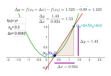
\includegraphics[width=0.48\textwidth]{math-insight.pdf}
  \end{wrapfigure}
  We investigate the benefits of virtual manipulatives and the
  influence of the support given to learners as they navigate online
  activities.

  \vspace{1ex}The event log resides in an open data warehouse, so 
  educational researchers can probe the data to generate additional
  knowledge on students learning.
\end{sectionblock}

    

    \end{column}%2

    %-- Column 3 ---------------------------------------------------
    \begin{column}{0.32\linewidth}
      \vspace{-2ex}\phantom{\makebox[0in][l]{\Large\textsf{Empowering faculty to run online learning experiments}}}
\vspace{1ex}

\begin{sectionblock}{DoenetML}

  \begin{wrapfigure}{L}{0.4\textwidth}
    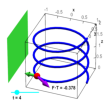
\includegraphics[width=0.38\textwidth]{vector-field.pdf}
  \end{wrapfigure}
  Interactives can be built via DoenetML, a semantic markup
  language built to enable authors to create virtual manipulatives for
  learners.
  % Interactives can be built via DoenetML, an opinionated markup
  % language built to encode learner interactions with mathematical
  % content.  Starting with primitives like \texttt{<point>}, complex
  % interactives can be described and then shared with learners.
\end{sectionblock}

\vspace{1ex}

\begin{sectionblock}{Doenet API}
  Webpages, whether or not they are written using DoenetML, can use
  the Doenet API to record events.  These events can be analyzed to
  understand how engagement with the webpage affects learning.
  
\end{sectionblock}

\vspace{1ex}

\begin{sectionblock}{Join the Ongoing Work}
  Instructors, curriculum designers, technologists, and educational
  researchers will be brought together at Doenet workshops to
  collaborate.

  \vspace{1ex}
  \setbeamercolor{callout}{fg=chocolate,bg=donut}
  \begin{beamercolorbox}[sep=0.5em]{callout}
    \vspace{1ex}\textbf{Contact us at \texttt{info@doenet.org} to join the
      ongoing effort.}
  \end{beamercolorbox}
\end{sectionblock}



    \end{column}
 
  \end{columns}
\end{frame}
}
\end{document}
